\documentclass[10pt,a4paper]{article}
\usepackage{amsmath}
\usepackage{amssymb}
\usepackage{amsthm}
\usepackage{enumerate}
\usepackage{fancyhdr}
\usepackage{graphicx}
\usepackage{hyperref}
\usepackage{caption}
\usepackage[utf8]{inputenc}
\usepackage[a4paper, top=1in, bottom=1.25in, left=0.75in, right=0.75in]{geometry}

\begin{document}
\pagestyle{fancy}
\fancyhead[R]{Robert Schüle 319782, Christoph Ende 331655}

%%%%%%%%%%%%%%%%%%%%%%%%%%%%%%%%%%%%%%%%%%%%%%%%%%%%%%%%%%%%%%%%%%%%%%%%%%%%%%%%
\subsection*{10.1 Directed Acyclic Graphs and Graphical Models}
\begin{enumerate}[a)]
	\item

		\begin{itemize}
			\item directed acyclic graphs consist of nodes which represent random variables and directed links representing the relationships between those random variables
			\item links reach from one node, called \textit{parent}, to another node, the \textit{child} which is statistically dependent of its parents (with probability distribution $P(x_i\,|\,\mbox{parents}(x_i))$)
		\end{itemize}

 \item

 		\begin{itemize}
	 		\item conditional independence means that two or more random variables are statistically independent, iff another event becomes true
			\item
 		\end{itemize}

 \item

 		\begin{itemize}
			\item there are several possibilities, e.g. the following: $\;F,\,E,\,B,\,A,\,D,\,H,\,C,\,G$
		\end{itemize}

 \item

	  \begin{itemize}
	 		\item factorisation: $P(X) \;=\; P(E)\,P(F)\,P(B)\,P(A|F)\,P(D|F,E,A)\,P(H|B,A)\,P(C|F,H)\,P(G|A,H)$
	 	\end{itemize}

 \item

    \begin{itemize}
		 	\item the Markov blanket consists of all parents, children and children's parents: $\;F,\,H,\,D,\,G,\,E,\,B$
		\end{itemize}

 \item

	  \begin{itemize}
	 		\item
	 	\end{itemize}

\end{enumerate}


%%%%%%%%%%%%%%%%%%%%%%%%%%%%%%%%%%%%%%%%%%%%%%%%%%%%%%%%%%%%%%%%%%%%%%%%%%%%%%%%
\subsection*{10.3 Construction of a DAG}
\begin{enumerate}[a)]
\item

\begin{itemize}
	\item the figure below shows a DAG based on the given random variables
	\item the event \textit{Alarm} can be caused by \textit{Burglary} and \textit{Earthquake} while the event \textit{Radio broadcast} can only be triggered by \textit{Earthquake}
\end{itemize}

	\begin{figure}[h]
  	\centering
    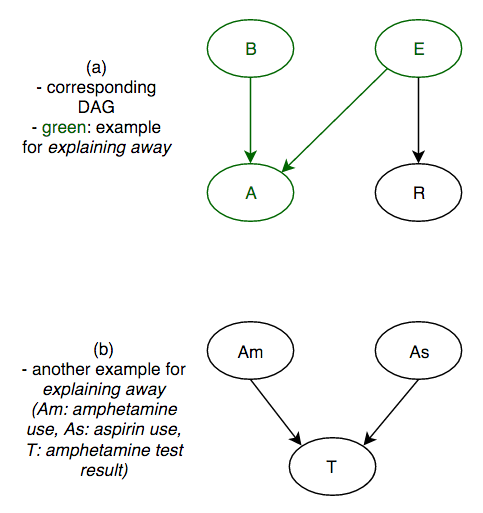
\includegraphics[width=0.5\textwidth]{103.png}
		\caption{DAG realisation of given random variables}
	\end{figure}

\item

		\begin{itemize}
			\item explaining away means that two statistically independent random variables can become statistically dependent by observing a common child
			\item
			\item
		\end{itemize}


\end{enumerate}

%%%%%%%%%%%%%%%%%%%%%%%%%%%%%%%%%%%%%%%%%%%%%%%%%%%%%%%%%%%%%%%%%%%%%%%%%%%%%%%%
\end{document}
